\documentclass{article}

% Language setting
% Replace `english' with e.g. `spanish' to change the document language
\usepackage[italian]{babel}

% Set page size and margins
\usepackage[a4paper,top=3cm,bottom=3cm,left=3cm,right=3cm,marginparwidth=1.75cm]{geometry}

% Useful packages
% \usepackage{showframe}
% \usepackage{layout}
%comando per più righe su una cella di tabella
\newcommand{\quantities}[1]{%
  \begin{tabular}{@{}c@{}}\strut#1\strut\end{tabular}%
}

\usepackage[dvipsnames, table]{xcolor}
\usepackage{amsmath}
\usepackage{graphicx}
\usepackage[colorlinks=true, allcolors=blue]{hyperref}
\usepackage{tikz}
\usetikzlibrary{shapes, backgrounds, mindmap, trees}
\usepackage{fancyhdr}
\usetikzlibrary{positioning}
\usepackage[inkscapeformat=png]{svg}

\usepackage{hyperref}
\usepackage{lastpage}
\usepackage{moresize}
\usepackage{paracol}
\usepackage{enumitem}
\usepackage{nicematrix}
\usepackage{tabularx}
\usepackage{parskip}
\usepackage{fontspec}
\usepackage{style}
\usepackage{float}
\usepackage{setspace}

\setmainfont{Poppins}[
    Path=./Poppins/,
    Extension = .ttf,
    UprightFont=*-Regular,
    BoldFont=*-Bold,
    ItalicFont=*-Italic,
    BoldItalicFont=*-BoldItalic
    ]

\title{Titolo}
\author{SWEetCode}

\begin{document}

\begin{titlepage}
    \thispagestyle{empty}
    \begin{tikzpicture}[remember picture, overlay]
        % TRIANGOLI
        \draw[fill=secondarycolor, secondarycolor] (current page.north west) -- (current page.south west) -- (8.8, -28);
        \draw[fill=primarycolor, primarycolor] (-3, 5) -- (4, -13.6) -- (11, 5);

        % LOGO
        \node [xshift=-5cm, yshift=25cm] (logo) at (current page.south east) {\includesvg[width=6.5cm]{logo.svg}};

        % SWEETCODE - DATE
        \node [anchor=north east, align=right, xshift=-1.2cm, yshift=20.5cm, text=black] (sweetcode) at (current page.south east) {\fontsize{32pt}{36pt}\selectfont SWEetCode};
        \draw[line width=4pt, lightcol] ([xshift=-3cm, yshift=-0.37cm]sweetcode.south west) -- ([yshift=-0.37cm]sweetcode.south east);
        \node [anchor=north east, align=right, xshift=-1.2cm, yshift=18.7cm, text=black] (date) at (current page.south east){\fontsize{24pt}{24pt} \selectfont 2023-11-08 };

        % NOME FILE
        \node [anchor=north east, text width=15cm, align=right, xshift=-1.2cm, yshift=17cm, text=black] (titolo) at (current page.south east){\fontsize{48pt}{48pt}\textbf{Valutazione capitolati}}; % andare a capo con \\

        % BOX DATI PARTECIPANTI
        \node[anchor=north east, xshift=-1.2cm, yshift=12cm, minimum width=8cm] (box) at (current page.south east){};

        % VERSIONE
        \node[anchor=north west, align=left] (dati1) at (box.north west) {\fontsize{16pt}{16pt}\selectfont \textbf{}};
        % \draw[line width=4pt, lightcol] (dati1.south west) -- ([xshift=8cm]dati1.south west);
        \node[anchor=north west, align=left] (dati11) at (dati1.south west)
        {\fontsize{14pt}{14pt}\selectfont};

        % COMPONENTI DEL GRUPPO
        \node[anchor=north west, yshift=-1cm, align=left] (dati2) at (dati11.north west) {\fontsize{16pt}{16pt}\selectfont \textbf{Componenti del gruppo}};
        \draw[line width=4pt, lightcol] (dati2.south west) -- ([xshift=8cm]dati2.south west);
        \node[anchor=north west, align=left] (dati21) at (dati2.south west)
        {\fontsize{14pt}{14pt}\selectfont Bresolin G.};
        \node[anchor=north west, yshift=-0.7cm, align=left] (dati22) at (dati2.south west)
        {\fontsize{14pt}{14pt}\selectfont Campese M.};
        \node[anchor=north west, yshift=-1.4cm, align=left] (dati23) at (dati2.south west)
        {\fontsize{14pt}{14pt}\selectfont Ciriolo I.};
        \node[anchor=north west, yshift=-2.1cm, align=left] (dati24) at (dati2.south west)
        {\fontsize{14pt}{14pt}\selectfont Dugo A.};
        \node[anchor=north west, yshift=-2.8cm, align=left] (dati25) at (dati2.south west)
        {\fontsize{14pt}{14pt}\selectfont Feltrin E.};
        \node[anchor=north west, yshift=-3.5cm, align=left] (dati26) at (dati2.south west)
        {\fontsize{14pt}{14pt}\selectfont Michelon R.};
        \node[anchor=north west, yshift=-4.2cm, align=left] (dati27) at (dati2.south west)
        {\fontsize{14pt}{14pt}\selectfont Orlandi G.};
        
        % UNIPD - SWE
        \node [xshift=4.4cm, yshift=2.3cm, draw, secondarycolor, text=white] (uni) at (current page.south west) {\fontsize{20pt}{20pt} \selectfont Università di Padova};
        \node [xshift=0.65cm, yshift=0.7cm, draw, secondarycolor, text=white, below=of uni] (corso) {\fontsize{20pt}{20pt}\selectfont Ingegneria del Software};

        % FIRMA
        % \draw[line width=4pt, lightcol] ([xshift=-1.2cm, yshift=1.8cm]current page.south east) -- ([xshift=-8cm, yshift=1.8cm]current page.south east);
        % \node[anchor=north west, xshift=12.9cm, yshift=1.45cm, align=left] at (current page.south west)
        % {\fontsize{13pt}{13pt}\selectfont L'Amministratore: Feltrin E.};
        
    \end{tikzpicture}
\end{titlepage}

%Registro in ordine dalla più recente alla meno recente!
{\renewcommand{\arraystretch}{1.5}
\section*{Registro delle versioni}
\begin{tabularx}{\textwidth}{c|c|c|c|X}
\textbf{Versione} & \textbf{Data} & \quantities{\textbf{Responsabile di}\\\textbf{stesura}}& \textbf{Revisore} & \quantities{\textbf{Dettaglio e}\\\textbf{motivazioni}} \\
\hline
v0.0.1(23) & $2023-11-13$ & Campese M. & Feltrin E. & Modifiche correttive di versione e registro delle modifiche. \\
\hline
v0.0.1(16) & $2023-10-29$ &  Michelon R. & Dugo A. & Correzioni e migliorie sintattiche.\\
\hline
v0.0.1(15) & $2023-10-28$ & Dugo A. & Campese M. & C-2, C-3, C-8.\\
\hline
v0.0.1(11) & $2023-10-27$ & Michelon R. & Bresolin G. & C-1, C-6, C-9.\\
\hline
v0.0.1(6) & $2023-10-26$ & Orlandi G. & Ciriolo I. &  C-1, C-5, C-7.\\
\end{tabularx}}
\newpage

\tableofcontents
\newpage

\section{C-1. Knowledge Management AI}
\begin{itemize}
    \item \textbf{Proponente:} AzzurroDigitale S.r.l.
    \item \textbf{Committenti:} Prof. Tullio Vardanega e Prof. Riccardo Cardin
\end{itemize}

\subsection{Riassunto}
Con l’avanzamento dell’Intelligenza Artificiale, sono emerse nuove soluzioni che offrono un approccio innovativo per problemi di knowledge management.


Rispetto a tecniche manuali di archiviazione, le soluzioni basate sull’AI riescono a estrarre e strutturare i dati automaticamente, identificando anche relazioni nascoste tra di essi. 
Un sistema di questo tipo potrebbe essere uno strumento utile a operatori e dipendenti per reperire in maniera semplice ed efficiente informazioni specifiche riguardo manuali, regolamenti e indicazioni aziendali.


Volendo sfruttare questa opportunità, l’azienda AzzurroDigitale propone di sviluppare una piattaforma web per la gestione (caricamento, consultazione, eliminazione) dei documenti e un chatbot basato sull’intelligenza artificiale, il cui compito è quello di rispondere a richieste fatte dagli utenti basandosi sui dati contenuti nei documenti caricati nel sistema.


Di seguito è illustrato uno schema generale del funzionamento del sistema.

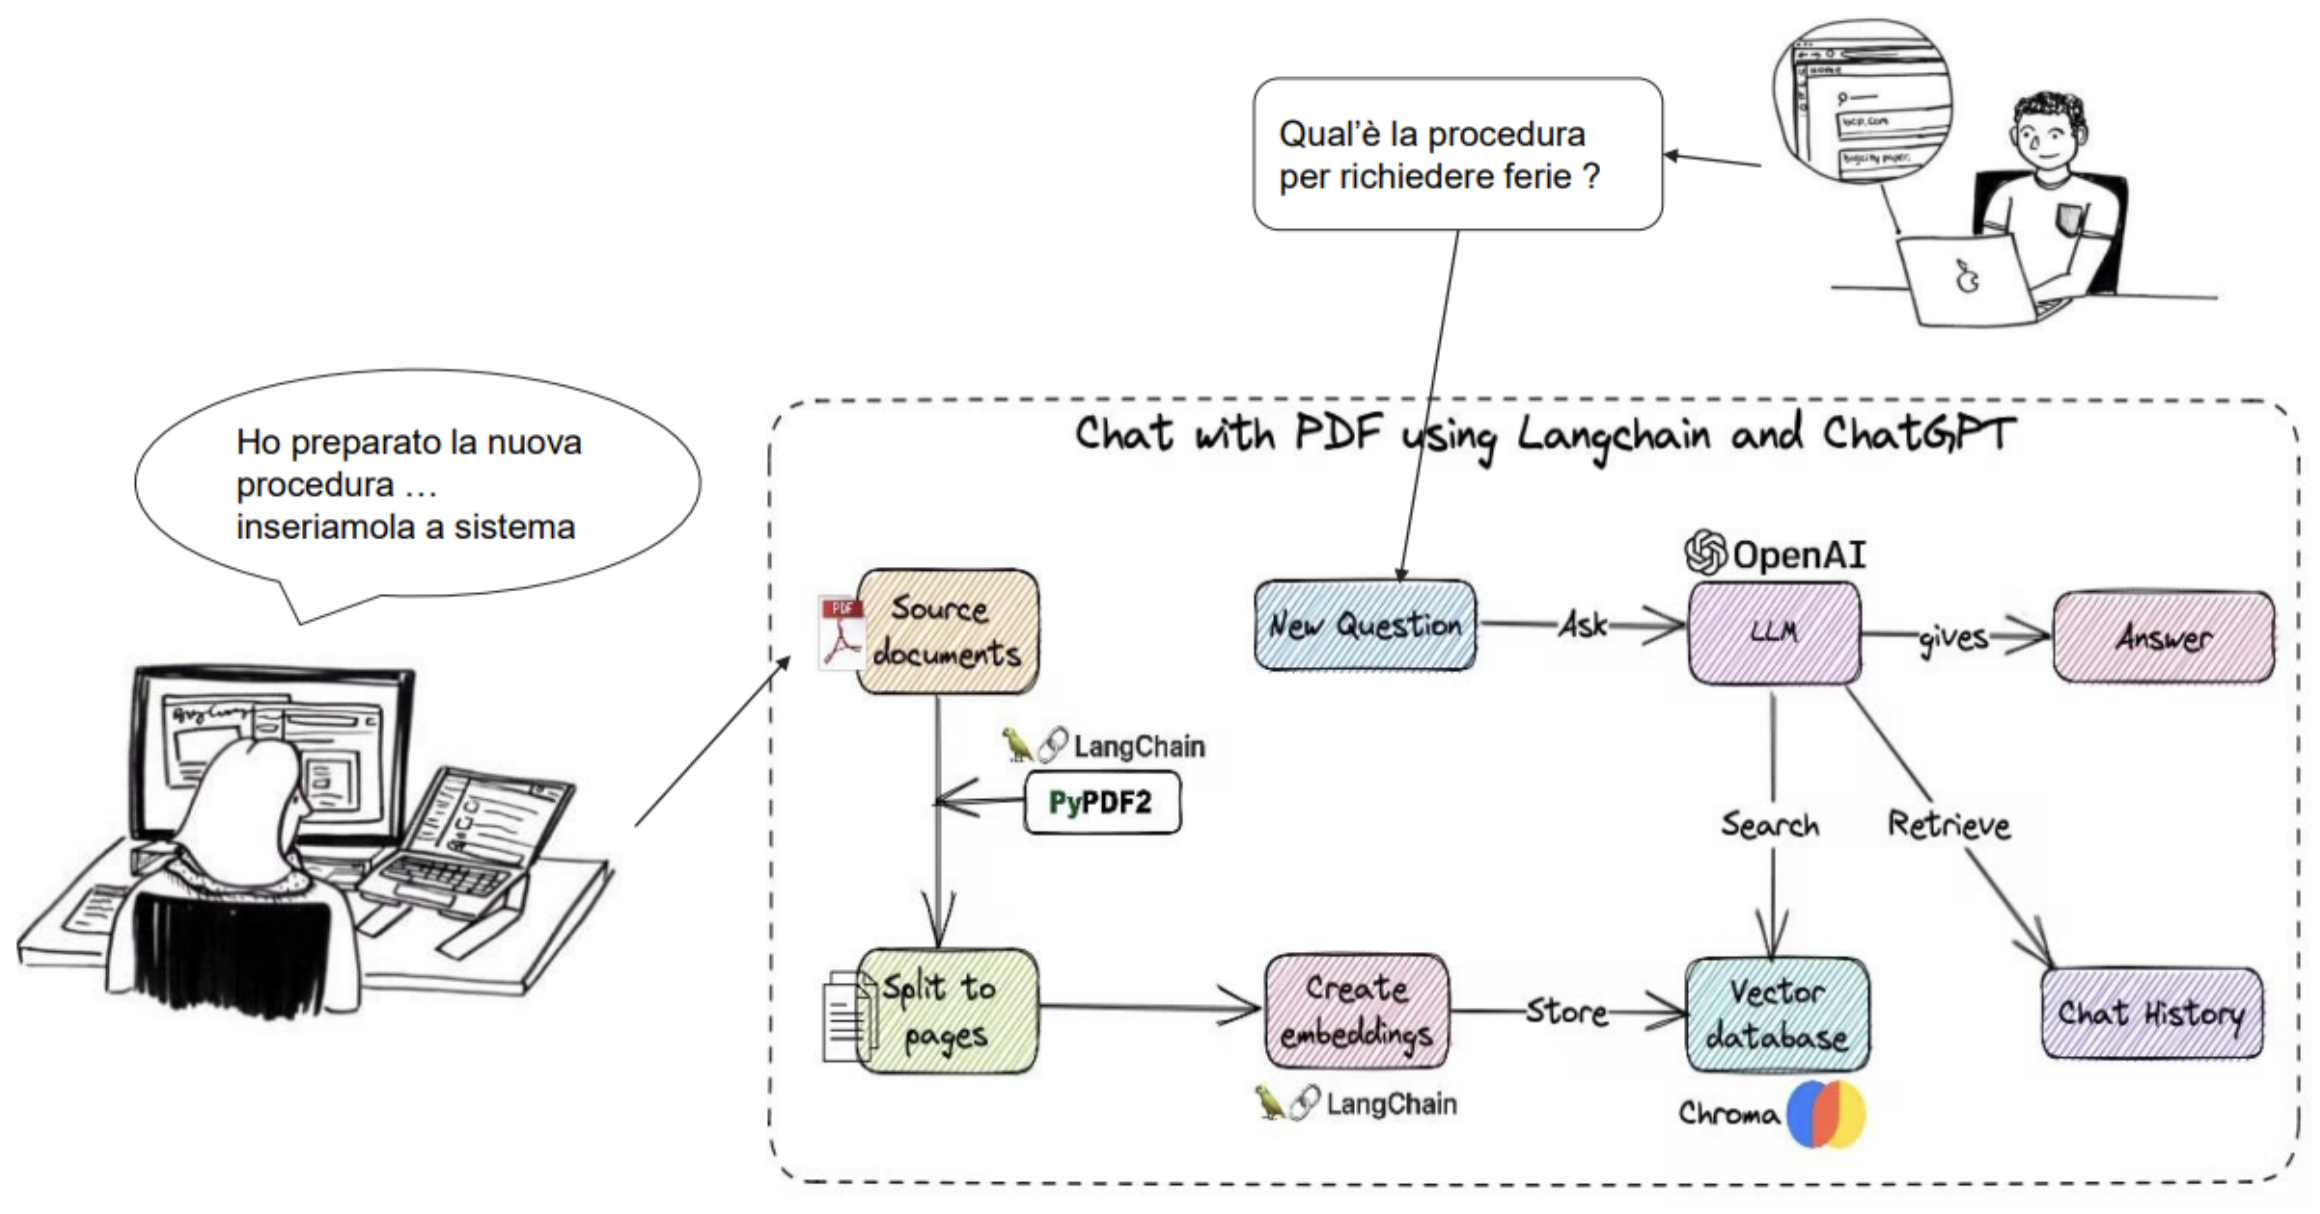
\includegraphics[width=1\textwidth]{Img_AD.png}

\subsection{Obiettivo}
Creare un sistema di Knowledge Management basato sull’AI per catturare, organizzare distribuire le conoscenze all'interno di un'organizzazione.
È richiesta la consegna del seguente materiale:
\begin{itemize}
    \item Documentazione tecnica: diagrammi di flusso, schemi di funzionamento, documentazione delle API;
    \item Bug reporting;
    \item Codice sorgente, raccolto in una repository git messa a disposizione dall’azienda.
\end{itemize}


\subsection{Dominio tecnologico}
\begin{itemize}
    \item \textit{Node.js}, runtime system per l’esecuzione di codice \textit{Javascript};
    \item \textit{Angular}, framework open-source \textit{Typescript} per sviluppare la UI front-end;
    \item \textit{OpenAI}, motore per le funzionalità di NLP (Natural Language Processing), tramite il quale viene elaborata la richiesta e generata una risposta opportuna;
    \item \textit{LangChain}, framework open-source che semplifica la comunicazione con modelli di AI, permette di collegare altre fonti di dati e offre funzionalità come document analysis, summarization, code analysis e l’implementazione di chatbot;
    \item \textit{Chroma}, un vector store open-source usato per la memorizzazione e il recupero di word embedding (o word vector) in modo efficiente.
\end{itemize}

\subsection{Aspetti Positivi}
\begin{itemize}
    \item Argomento e tecnologie interessanti, sempre più utilizzate e richieste nel mondo del lavoro;
    \item Progetto che ha uno scopo ben preciso e delineato, con fini socialmente utili;
    \item Ottime tecnologie, supportate da una grande community;
    \item Flessibilità nella scelta delle tecnologie da utilizzare.
\end{itemize}
\subsection{Aspetti Negativi}
\begin{itemize}
    \item Presentazione non molto dettagliata che omette alcuni dettagli implementativi.
\end{itemize}

\subsection{Conclusioni}
Sin da subito il capitolato proposto da AzzurroDigitale è stato apprezzato dall’intero gruppo e il successivo incontro effettuato con l’azienda ha confermato l’interesse. Per queste ragioni oltre che agli aspetti positivi precedentemente citati, dopo un’attenta votazione, il gruppo ha deciso di scegliere C-1 come prima preferenza.

\newpage
\section{C-2. Sistema di Raccomandazione}
\begin{itemize}
    \item \textbf{Proponente:} Ergon Informatica S.r.l.
    \item \textbf{Committenti:}  Prof. Tullio Vardanega e Prof. Riccardo Cardin
\end{itemize}

\subsection{Riassunto}
Il progetto in questione è applicabile a imprese il cui principale focus aziendale è la commercializzazione di prodotti. Queste aziende eseguono campagne di marketing e piani commerciali per promuovere prodotti o incrementare le vendite adottando principalmente due strategie: una ad ampio spettro ed una mirata.

Grazie al possesso e l’analisi dei dati storici dei clienti, l’azienda sarà in grado di raggrupparli in base a similitudini e scoprire interessi non evidenti dai loro acquisti passati.
Il progetto mira a creare un sistema che consigli all'azienda come indirizzare specifiche iniziative di marketing e commerciali, identificando gruppi di clienti target.
Il sistema di raccomandazione utilizzerà feedback che potranno essere espliciti o impliciti. La sua implementazione invece potrà avvenire in uno dei seguenti modi: collaborative filtering oppure content-based filtering.

Il sistema proposto è riassunto nel seguente schema.\\
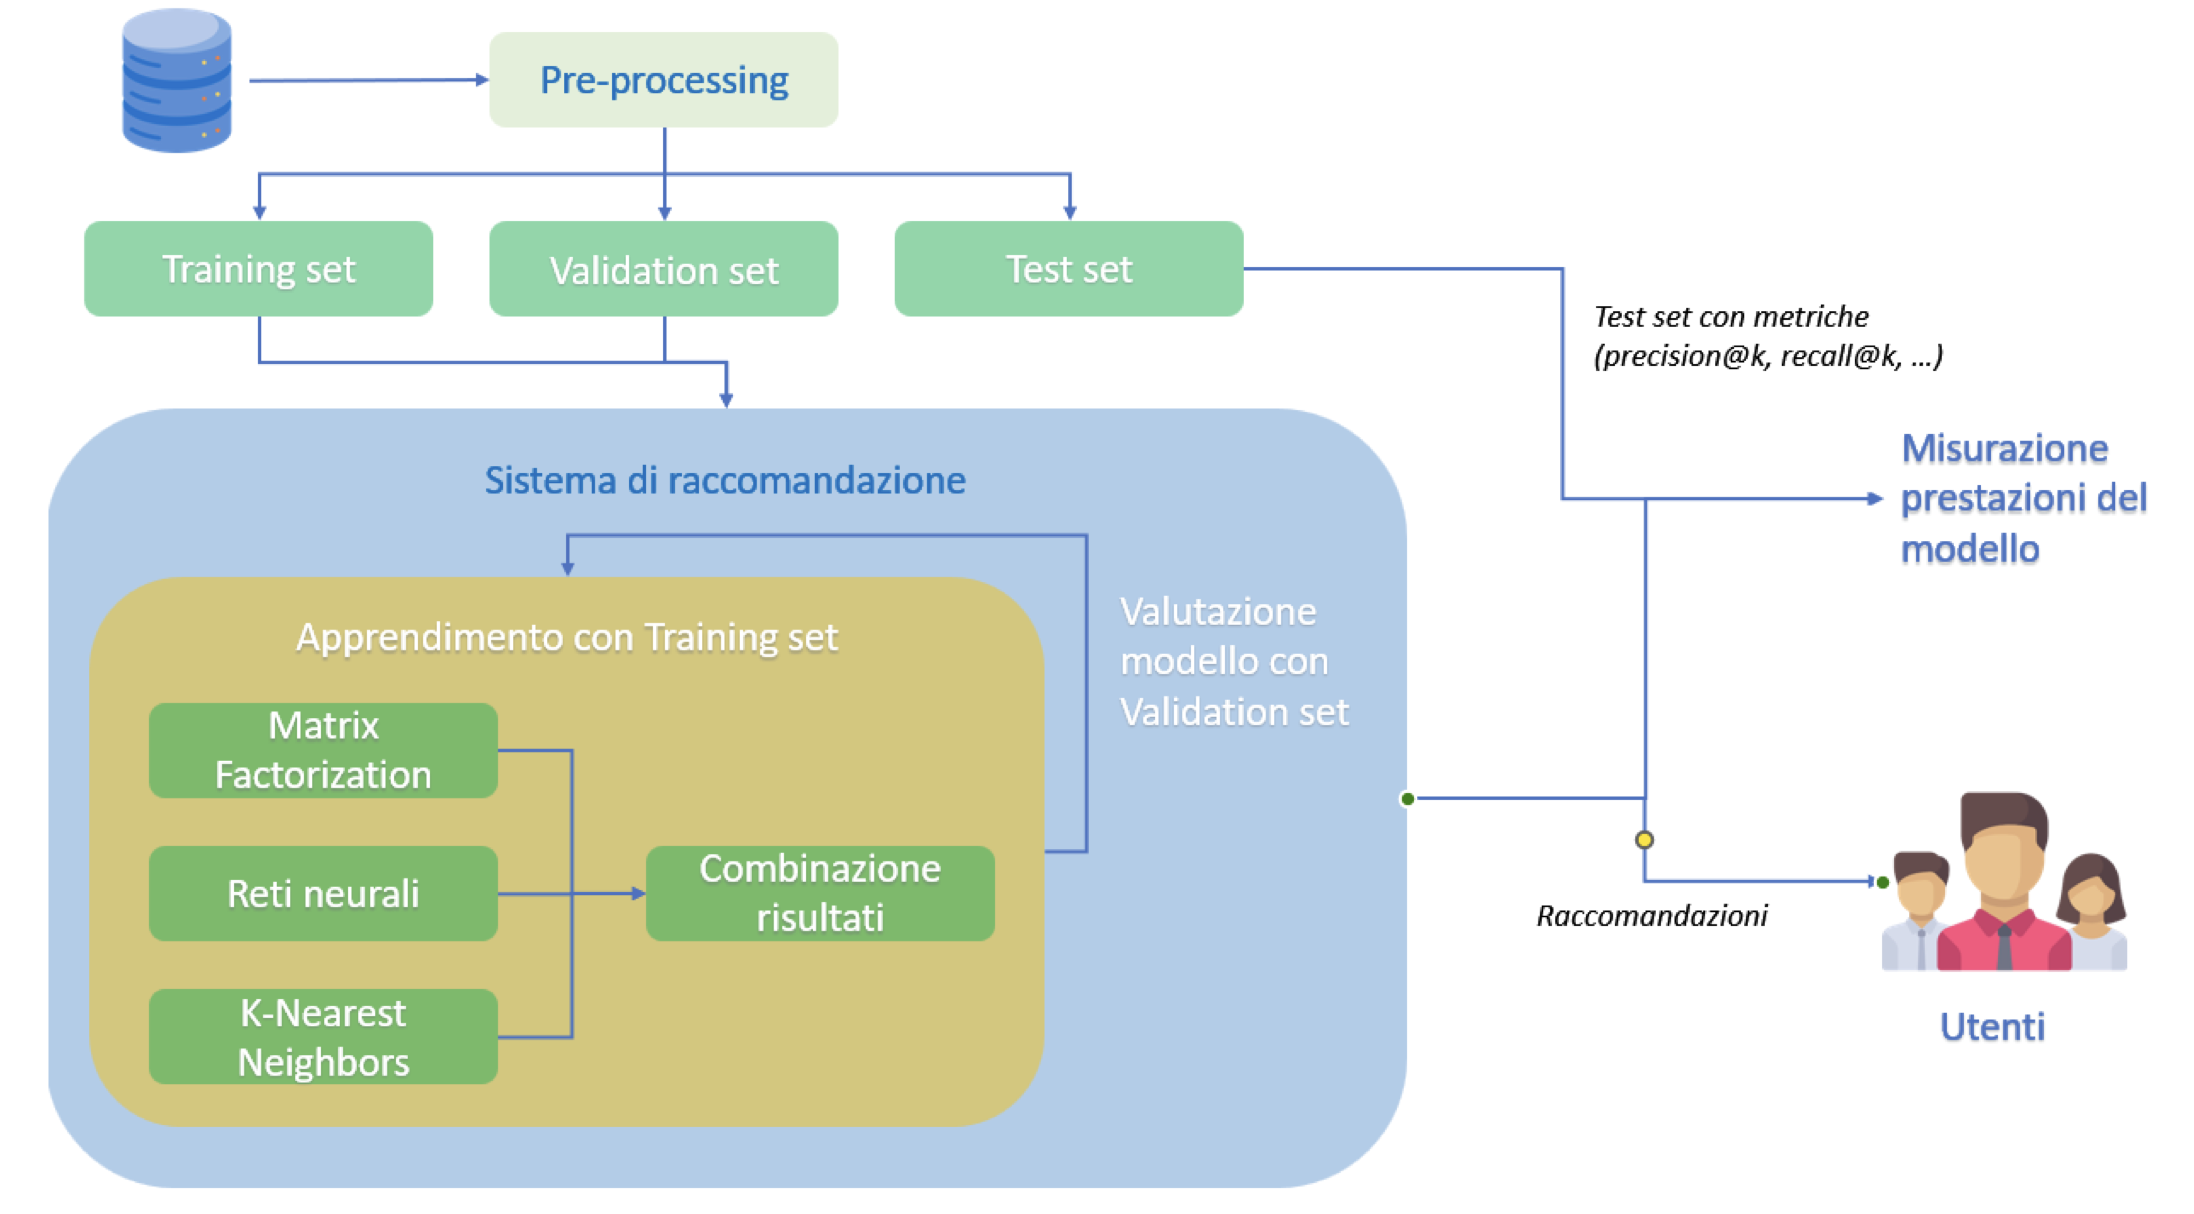
\includegraphics[width=1\textwidth]{im_ERGON.png}


\subsection{Obiettivo}
Realizzare un Sistema di Raccomandazione basato sull'Intelligenza Artificiale per orientare le attività aziendali, suggerendo su quali clienti dovrebbero essere mirate le iniziative di marketing.
In particolare la piattaforma da sviluppare dovrà essere formata dai seguenti componenti:

\begin{itemize}
    \item Database relazionale per la gestione dei dati;
    \item Motore di raccomandazione;
    \item Interfaccia utente, UI desktop-based o web-based, per la consultazione dei risultati e ritorno di feedback degli utenti.
\end{itemize}

\subsection{Dominio tecnologico}
\begin{itemize}
    \item \textit{SQL Server Express, MySql o MariaDB};
    \item \textit{ML.NET} (basato su framework \textit{.NET} utilizzando il linguaggio \textit{C\#}) o \textit{Surprise} (libreria \textit{Python}).
\end{itemize}

\subsection{Aspetti Positivi}
\begin{itemize}
    \item libertà di scelta per le tecnologie da utilizzare;
    \item Il materiale informativo proposto è molto approfondito e l’incontro con l’azienda ha dimostrato una buona conoscenza nell’ambito tecnologico proposto;
    \item Proposta di formazione da parte dell’azienda.
\end{itemize}

\subsection{Aspetti Negativi}
\begin{itemize}
    \item Tecnologie proposte hanno un basso learning rate.
\end{itemize}
\subsection{Conclusioni}
Sebbene le buone impressioni legate al capitolato siano state confermate dall’incontro, le tecnologie proposte ci hanno fatto virare verso altre opzioni. Dopo una fase di votazione, il gruppo ha deliberato di designare questo capitolato come terza scelta.

\newpage

\section{C-3. EasyMeal}
\begin{itemize}
    \item \textbf{Proponente:} Imola Informatica
    \item \textbf{Committenti:}  Prof. Tullio Vardanega e Prof. Riccardo Cardin
\end{itemize}

\subsection{Riassunto}
EasyMeal semplifica radicalmente il processo di prenotazione nel settore dei ristoranti, consentendo agli utenti di riservare un tavolo in modo intuitivo e rapido. 
Gli utenti inoltre potranno creare il proprio ordine da casa o dall'ufficio, personalizzandolo in base alle proprie esigenze, allergie e preferenze alimentari.
EasyMeal offre anche un'esperienza di ordine coinvolgente e collaborativa. I clienti infatti potranno interagire direttamente con lo staff del ristorante per chiedere informazioni sulle pietanze e monitorare gli ordini degli altri membri del loro tavolo.
Attraverso l'app si potrà anche dividere il conto tra i partecipanti, semplificando ulteriormente la gestione delle spese nei gruppi.

\subsection{Obiettivo}
Sviluppare un’applicazione web responsive (EasyMeal) per semplificare il processo di prenotazione e ordinazione delle pietanze direttamente da remoto.
Applicazione web responsive (PC, \textit{IOS} e \textit{Android}) con:

\begin{itemize}
  \item Sistema di registrazione utenti (registrazione, login e logout);
  \item Consultare la lista di ristoranti con sistema di filtraggio per data, orario, città e tipologia di cucina;
  \item Collegamento di una prenotazione ad un ristorante e all’ordinazione creata dagli utenti di un tavolo;
  \item Chat privata tra utente e amministratore del ristorante;
  \item Notifiche agli utenti e agli amministratori dei ristoranti;
  \item Interazione con lo staff del ristorante;
  \item Pagamento di un conto;
  \item Consultazione delle prenotazioni da parte di un amministratore del ristorante;
  \item Inserimento di feedback e recensioni;
  \item Notifiche per amministrazione e utenti;
  \item Sistema di pagamento.
\end{itemize}


\subsection{Dominio tecnologico}
Assenti.

\subsection{Aspetti Positivi}
\begin{itemize}
    \item L’azienda non propone nessuna tecnologia da utilizzare, lasciando totale libertà nella scelta implementativa;
    \item Funzionalità che prese singolarmente non risultano complesse.
\end{itemize}

\subsection{Aspetti Negativi}
\begin{itemize}
    \item Progetto con molte funzionalità e casi d’uso, la cui implementazione risulta complessa;
    \item L’argomento non presenta niente di innovativo.
\end{itemize}
\subsection{Conclusioni}
La proposta non ha suscitato interesse da parte dei componenti del gruppo, quindi non è stata inserita tra le possibili scelte del gruppo.

\newpage

\section{C-4. ChatGPT plugin con Nuvolaris serverless}
\begin{itemize}
    \item \textbf{Proponente:} Nuvolaris
    \item \textbf{Committenti:}  Prof. Tullio Vardanega e Prof. Riccardo Cardin
\end{itemize}

\subsection{Riassunto}
Il progetto che l’azienda propone si basa sulla creazione di un plugin per una delle loro produzioni software, chiamato \textit{Nuvolaris}, un servizio per lo sviluppo in cloud serverless e \textit{FaaS} (Function-as-a-Service). 
\textit{FaaS} è un tipo di servizio di cloud computing basato su eventi ed eseguito in container stateless che consente agli sviluppatori di creare, eseguire e gestire i pacchetti applicativi come funzioni, senza dover mantenere un'infrastruttura propria.
Tramite \textit{Nuvolaris} è possibile creare API e plugin scalabili, cioè capaci di aumentare o diminuire di scala in funzione delle necessità e disponibilità.


\subsection{Obiettivo}
Sviluppare un plugin di \textit{ChatGPT} per costruire app di una specifica categoria, ad esempio CRUD app con \textit{SQL} database, eCommerce app, forms come \textit{Google Forms}, e molto altro.
In particolare, vengono presentate le seguenti richieste:

\begin{itemize}
  \item Creare un template per un tipo di applicazione utilizzando file di configurazione;
  \item API per modificare e aggiornare il file di configurazione;
  \item Sistema per ricostruire l’applicazione basandosi sul file di configurazione. L’app deve essere live dopo ogni richiesta e deve essere generata usando funzioni serverless.

\end{itemize}


\subsection{Dominio tecnologico}
\begin{itemize}
    \item \textit{Nuvolaris}
    \item \textit{ChatGPT API}
\end{itemize}

\subsection{Aspetti Positivi}
\begin{itemize}
    \item L’azienda fornisce materiali utili come \textit{Nuvolaris} environment in Cloud, un account \textit{ChatGPT Pro}, documentazione relativa alle tecnologie proposte, supporto tramite \textit{Slack}.
\end{itemize}

\subsection{Aspetti Negativi}
\begin{itemize}
    \item Complesso da progettare idealmente;
    \item Proposta non chiara, soprattutto la descrizione del loro prodotto;
    \item Obbligo di utilizzo di una tecnologia proprietaria, sconosciuta al team;
    \item Non è ben specificato cosa intendono con template di app e che tipo di informazioni dovrebbe contenere un file di configurazione.
\end{itemize}
\subsection{Conclusioni}
Proposta non interessante per il gruppo, non considerata nelle preferenze.

\newpage

\section{C-5. WMS3: warehouse management 3D}
\begin{itemize}
    \item \textbf{Proponente:} Sanmarco Informatica SPA
    \item \textbf{Committenti:}  Prof. Tullio Vardanega e Prof. Riccardo Cardin
\end{itemize}

\subsection{Riassunto}
Un Warehouse Management System (WMS) ha come obiettivo principale la tracciabilità e il controllo dello stoccaggio nei magazzini, supervisionando il loro flusso, gestendo tutte le operazioni, dal ricevimento dei beni alla loro spedizione o all'utilizzo nei relativi reparti di produzione. Questo tipo di sistema è progettato per assicurare che le richieste di prelievo vengano evase puntualmente e per massimizzare l'efficiente utilizzo degli spazi fisici nel magazzino.
I principali obiettivi di un sistema WMS sono il controllo delle performance, la razionalizzazione dei costi e l'ottimizzazione dei processi di logistica. 

Per fare ciò è preferibile implementare un’esperienza 3D che rappresenta il magazzino e tutti i suoi reparti, con lo scopo di massimizzare la visibilità e migliorare l’esperienza utente.

Di seguito alcune raccomandazioni esplicite suggerite da Sanmarco Informatica SPA:
\begin{itemize}
    \item Nessun login;
    \item Sessioni volatili (no persistenza delle modifiche, quali l’ultima posizione visionata);
    \item Solo gestione “amministratore”;  
    \item Non è richiesta l’integrazione con sistemi di VR;
    \item Contatti frequenti gruppo di lavoro - proponente.
\end{itemize}
\subsection{Obiettivo}
Gestire correttamente il magazzino come chiave per raggiungere l’efficienza dei flussi e dei processi aziendali.
In particolare, sono state presentate le seguenti richieste:

\begin{itemize}
    \item Sviluppare un'applicazione che offra un'area 3D in cui sia possibile aggiungere manualmente scaffalature e modificarle a piacimento;
    \item Fornire la possibilità di codificare le coordinate della scaffalatura in righe e colonne per identificare le aree disponibili in cui posizionare gli oggetti;
    \item Consentire agli utenti di selezionare un prodotto (oggetto all'interno della scaffalatura) e richiederne lo spostamento in un'area diversa;
    \item Consentire il caricamento di un'immagine \textit{SVG} da utilizzare come base della struttura;
    \item Implementare il precaricamento del layout del magazzino da un database;
    \item Offrire la possibilità di posizionare gli oggetti in coordinate specifiche o di evidenziare un prodotto cercato.
\end{itemize}


\subsection{Dominio tecnologico}
\begin{itemize}
    \item \textit{Three.js} (\textit{Javascript}) (consigliate);
    \item \textit{Unity} (\textit{C\#}), \textit{Unreal Engine} (\textit{C++}) (alternative)
\end{itemize}

\subsection{Aspetti Positivi}
\begin{itemize}
    \item Documentazione proposta è visivamente molto curata, con esempi visuali che illustrano una possibile implementazione della proposta.
\end{itemize}

\subsection{Aspetti Negativi}
\begin{itemize}
    \item Tecnologie complesse che non sono risultate interessanti a tutti i componenti del gruppo;
    \item Non molto chiare le modalità di inserimento e spostamento del materiale di stoccaggio.
\end{itemize}
\subsection{Conclusioni}
L’argomento e l’ambito di applicazione del progetto non sono stati fonte di motivazione ed interesse per i membri del gruppo.



\newpage



\section{C-6. SyncCity (Smart City Monitoring Platform)}
\begin{itemize}
    \item \textbf{Proponente:} Sync Lab S.r.l.
    \item \textbf{Committenti:}  Prof. Tullio Vardanega e Prof. Riccardo Cardin
\end{itemize}
\subsection{Riassunto}
Sync Lab propone di sviluppare un sistema che riesca a simulare nel modo più realistico possibile i dati dei sensori di misurazione di una città, rappresentandoli in una serie di dashboard.
I dati dovranno essere simulati attraverso tool di generazione di informazioni random, ma qualora ci fosse l’opportunità di raccoglierli da fonti esterne reali, l’azienda potrebbe discuterne l’utilizzo.

La città monitorata potrebbe essere suddivisa in celle e per ognuna di esse potrebbero essere prese varie sorgenti di dati, come ad esempio: informazioni atmosferiche, inquinamento, traffico, lavori di manutenzione, guasti, criticità strutturali e molto altro.

La piattaforma dovrà raccogliere questi dati e salvarli su una piattaforma \textit{OLAP} (On-Line Analytical Processing), permettendo agli utenti di visualizzarli in dashboard dedicate.

\subsection{Obiettivo}
Realizzare una piattaforma e relativa dashboard che consenta a chi la usa di avere sotto controllo una serie di informazioni sullo stato di salute della città, in modo da prendere decisioni veloci, efficaci ed analizzare poi gli effetti conseguenti.


\subsection{Dominio tecnologico}
\begin{itemize}
    \item \textit{Faker} di \textit{Python}, framework per la simulazione dei dati;
    \item \textit{Apache Kafka}, broker per disaccoppiare lo stream di informazioni provenienti dai diversi simulatori;
    \item \textit{ClickHouse}, database \textit{OLAP} che mantiene la persistenza di dati con numerosità elevata;
    \item \textit{Grafana}, piattaforma di data visualization per la creazione di diagrammi e grafici, raccolti in dashboard.
\end{itemize}

\subsection{Aspetti Positivi}
\begin{itemize}
    \item Dominio tecnologico proposto considerato molto interessante e attuale.

\end{itemize}

\subsection{Aspetti Negativi}
\begin{itemize}
    \item Integrazione complessa tra tutte le tecnologie proposte;
    \item La proposta di simulare la generazione dei dati ricevuti dal sistema, seppur presentata come semplificazione, ha rimosso l’entusiasmo iniziale del gruppo.

\end{itemize}
\subsection{Conclusioni}
Nonostante la proposta originale e il dominio applicativo sempre più richiesto, il gruppo ha optato per altri progetti ritenuti complessivamente più interessanti.


\newpage
\section{C-7. ChatGPT vs BedRock developer Analysis}
\begin{itemize}
    \item \textbf{Proponente:} Sync Lab S.r.l.
    \item \textbf{Committenti:}  Prof. Tullio Vardanega e Prof. Riccardo Cardin
\end{itemize}

\subsection{Riassunto}
Zero12 propone di creare un middleware che riceva in input dei requisiti di business e produca epic e user stories associate ai requisiti di business, comparando la capacità di \textit{ChatGPT} e quella di \textit{AWS BedRock} nell’interpretare del codice sorgente ed associare le user stories generate.
Il team dovrà svolgere un’analisi sulle \textit{API} di \textit{ChatGPT} e \textit{BedRock}, studiandone un approccio modulare che permette un uso alternativo dei due sistemi di Generative AI.


\subsection{Obiettivo}
\begin{itemize}
    \item Creare un plugin per \textit{Visual Studio Code};
    \item Creare un plugin per \textit{Apple Xcode};
    \item Confrontare i risultati forniti dal sistema utilizzando \textit{ChatGPT} e \textit{BedRock}.
\end{itemize}


\subsection{Dominio tecnologico}
\begin{itemize}
    \item \textit{AWS Fargate}: un servizio serverless per la gestione di container;
    \item \textit{MongoDB}: un database documentale ideale per la gestione di progetti basati su eventi;
    \item \textit{Node.js}: utilizzato per lo sviluppo di \textit{API REST} in formato \textit{JSON};
    \item \textit{Python}: utilizzato come plugin per \textit{Xcode};
    \item \textit{TypeScript}: utilizzato come plugin per \textit{Visual Studio Code} (\textit{VSCode});
    \item  \textit{API ChatGPT}: una interfaccia di programmazione applicativa per l'accesso al modello di linguaggio GPT-3;
    \item \textit{AWS Bedrock}: un framework o servizio di \textit{AWS} utilizzato nel progetto.
\end{itemize}


\subsection{Aspetti Positivi}
\begin{itemize}
    \item Il progetto risulta interessante e le tecnologie proposte sono state gradite dal gruppo;
    \item L’azienda è sembrata molto disponibile, offrendo varie proposte di supporto, tra cui una sessione di design thinking, seguita da guide sulla creazione dei requisiti di business, formazione sull’uso di tecnologie cloud \textit{Amazon Web Services}, sessioni tecniche di review del lavoro svolto;
    \item Offerta di fornitura di repository \textit{GIT}, \textit{Jira}, crediti i e account \textit{ChatGPT}.
\end{itemize}

\subsection{Aspetti Negativi}
\begin{itemize}
    \item Rispetto alla creazione di un intero sistema, la creazione di plugin non ha suscitato interesse ad alcuni componenti del gruppo;
    \item Non sono chiari i criteri di confronto dei due sistemi di AI.
\end{itemize}
\subsection{Conclusioni}
L’interesse per questo progetto non era condiviso da tutti i componenti del gruppo. Dopo una fase di votazione, il gruppo ha deciso di abbandonare la proposta.

\newpage

\section{C-8. JMAP}
\begin{itemize}
    \item \textbf{Proponente:} Zextras
    \item \textbf{Committenti:}  Prof. Tullio Vardanega e Prof. Riccardo Cardin
\end{itemize}

\subsection{Riassunto}
Il prodotto principale dell'azienda proponente è \textit{Carbonio}, un software per la collaborazione online on-premise che viene rilasciato come pacchetto installabile nell'infrastruttura server del cliente.
Attualmente, Carbonio basa il proprio servizio email su vari protocolli standard, tra cui \textit{IMAP}, \textit{POP} e \textit{Exchange ActiveSync}. Tuttavia, questi protocolli presentano diverse limitazioni, tra cui:

\begin{itemize}
    \item Non sono estendibili, il che vincola le funzionalità di Carbonio a ciò che offrono questi standard;
    \item Le funzionalità del calendario e dei contatti non sono erogate tramite un protocollo specifico, ma attraverso chiamate non standard basate su protocollo \textit{SOAP};
    \item L'uso di licenze \textit{ActiveSync} richiede il pagamento di onerosi diritti a \textit{Microsoft}.
\end{itemize}

Il protocollo di posta elettronica open-source \textit{JMAP}, a differenza dei protocolli citati precedentemente, è stato concepito con l'obiettivo di ottimizzare lo scambio di dati tra client e server, migliorando le prestazioni delle applicazioni attraverso richieste e risposte ottimizzate.
\textit{JMAP} utilizza il formato \textit{JSON} e definisce un set di API che permette ai client di accedere ai dati e gestirli in modo efficiente.
Sfruttando i meccanismi di sincronizzazione efficienti su cui si basa, \textit{JMAP} consente a più client di comunicare con il server in modo che le modifiche vengano visualizzate simultaneamente. Inoltre, \textit{JMAP} è progettato per essere estendibile, consentendo l'aggiunta di nuove funzionalità senza la necessità di modificare il protocollo di base.



\subsection{Obiettivo}
Capire se ha senso estendere \textit{Carbonio} aggiungendo la possibilità di utilizzare il protocollo \textit{JMAP}, mantenendo i vecchi standard per compatibilità con i client attualmente supportati, ma permettendo all’azienda di espandere le funzionalità offerte ai client di nuova generazione, offrendo anche uno standard implementativo alla versione \textit{Open Source} di \textit{Carbonio}.
L’azienda propone quindi di sviluppare un servizio di demo testabile con uno dei client pubblicizzati nel sito web ufficiale di \href{https://jmap.io/software.html)}{JMAP}
Questo servizio verrà poi utilizzato internamente a Zextras (assieme agli stress test che opzionalmente verranno forniti dal gruppo) per valutare le prestazioni, la manutenibilità e la completezza del protocollo \textit{JMAP}, paragonandolo agli attuali protocolli attualmente sviluppati in \textit{Carbonio}.
Seguono i requisiti funzionali esposti dall’azienda:
\begin{itemize}
    \item Invio e la ricezione di una mail;
\item Gestione delle cartelle;
\item Gestione dei contenuti di una cartella;
\item Eliminazione di un oggetto;
\item Eliminazione di una cartella;
\item Condivisione di una cartella;
\item Eliminazione di una condivisione di cartella.
\end{itemize}



\subsection{Dominio tecnologico}
 Nell'implementazione del protocollo \textit{JMAP} per il servizio \textit{Carbonio}, sono state stabilite le seguenti specifiche tecniche aggiuntive:
\begin{itemize}
    \item Linguaggio a scelta del gruppo di lavoro, con preferenza per \textit{Java} (essendo il linguaggio principale dello stack tecnologico di Carbonio);
    \item Libreria \textit{INPUTmice/JMAP} per l’implementazione del protocollo \textit{JMAP}. Alternativamente nel caso si scelga di optare per un linguaggio diverso, utilizzare l’implementazione presente in uno dei progetti elencati qui \textit{JMAP} Software Implementations per sviluppare la propria soluzione;
    \item Eseguibile in un sistema container, come \textit{Docker}. Questo ci permette di poter lanciare in maniera molto semplice una o più istanze del servizio, permettendoci di eseguire in batteria test di funzionalità e di performance;
    \item Deve essere scalabile mediante l’inizializzazione di più nodi stateless. Per stateless si intende che alla richiesta di uno specifico client fatta ad un’architettura contenente più di un’istanza del servizio dato, può rispondere una qualsiasi istanza del servizio, perché nessuna istanza contiene dati specifici di stato rispetto alle richieste dei client.
\end{itemize}

\subsection{Aspetti Positivi}
\begin{itemize}
    \item Proposta originale che permette di esplorare campi tecnologici non profondamente conosciuti dal gruppo;
\item Prodotto di utilizzo reale e utile in ambito applicativo per l’azienda.
\end{itemize}

\subsection{Aspetti Negativi}
\begin{itemize}
    \item Non chiaro il metodo di integrazione del protocollo \textit{JMAP} con il loro prodotto interno Carbonio
\end{itemize}
\subsection{Conclusioni}
Il capitolato in questione è stato scartato poiché tutti i membri del gruppo hanno manifestato opinioni negative a riguardo.








\newpage

\section{C-9. ChatSQL}
\begin{itemize}
    \item \textbf{Proponente:} Zucchetti
    \item \textbf{Committenti:}  Prof. Tullio Vardanega e Prof. Riccardo Cardin
\end{itemize}

\subsection{Riassunto}
Il “prompt engineering” è un processo di strutturazione del testo interpretato da modelli generativi di Intelligenza Artificiale.
Attraverso questo processo è possibile formulare dei prompt che guidano i modelli di AI nella produzione di risposte di maggiore qualità e coerenza tramite la scelta della sintassi, della struttura e del contesto, descritti in linguaggio naturale.
Il problema proposto consiste nella scrittura di frasi SQL a partire dalla definizione della struttura del database e della specifica della frase in linguaggio naturale.
In particolare, l’azienda chiede di sviluppare una applicazione che svolga i seguenti compiti:


\begin{itemize}
    \item Archiviazione della descrizione della struttura di un database, possibilmente commentata in tutte le sue parti. Questo può essere fatto sia tramite informazioni strutturate, che attraverso documenti di testo;
    \item Maschera di richiesta di una frase di interrogazione del database in linguaggio naturale, realizzabile attraverso un semplice campo di testo;
    \item Procedura che combina la richiesta di interrogazione con le informazioni della struttura del database creando un “prompt” che, sottoposto ad un sistema di AI, fornisce l’interrogazione equivalente al linguaggio naturale in linguaggio \textit{SQL}.
\end{itemize}

I tre punti precedenti devono essere integrati in un unico sistema che permetta di utilizzarli in modo integrato. L’intero sistema può essere riassunto dal seguente schema.\\
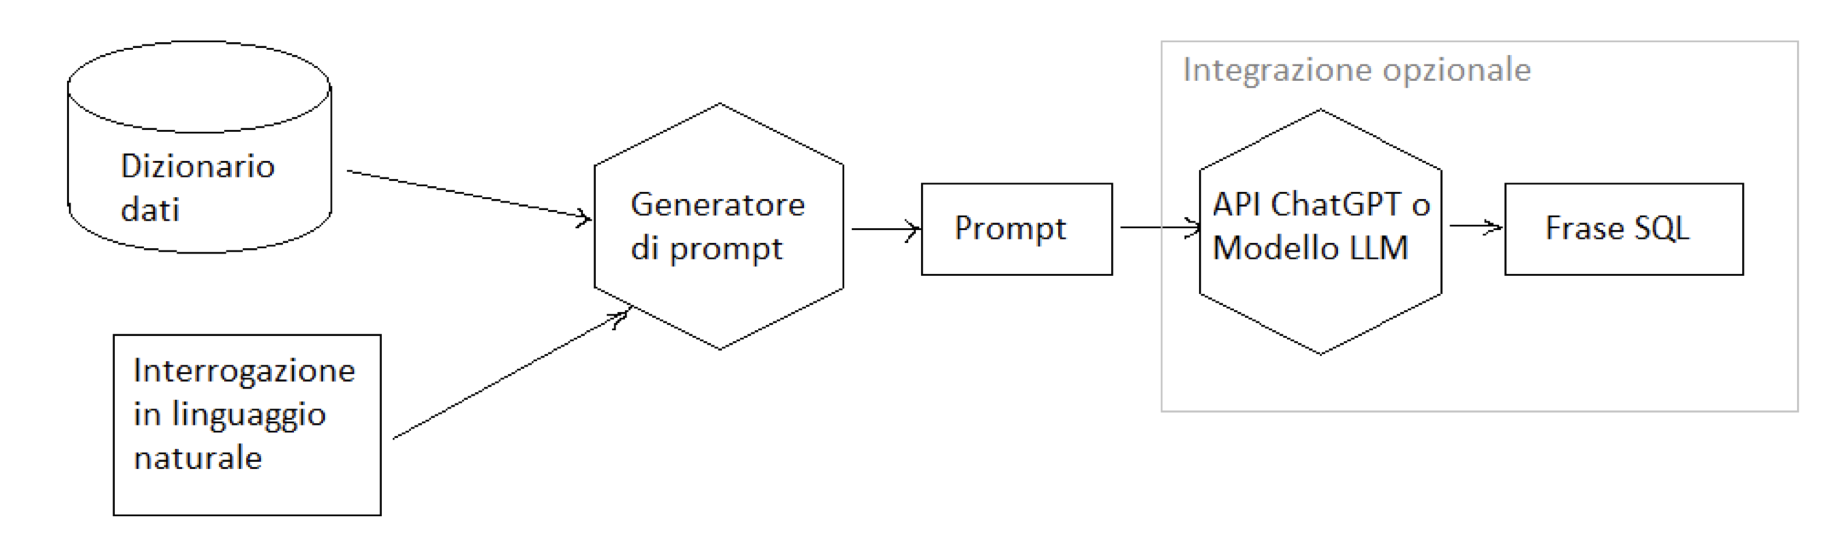
\includegraphics[width=1\textwidth]{img_Zucc.png}

Requisiti opzionali:

\begin{itemize}
    \item Visualizzare la frase \textit{SQL} prodotta dal sistema di AI;
    \item Sviluppare l’input vocale della frase in linguaggio naturale;
    \item Verificare la correttezza della frase \textit{SQL} prodotta dal sistema di AI tramite batterie di testing;
    \item Implementare la gestione di più basi di dati, archiviando diversi scenari e scegliendo quello opportuno nel momento in cui avviene una richiesta;
    \item Utilizzare modelli LLM alternativi a \textit{ChatGPT} (Es: \textit{Palm, LLaMa, Falcon});
    \item Addestrare un modello in modo specifico per la traduzione di frasi di interrogazione in italiano a frasi \textit{SQL}.
\end{itemize}


\subsection{Obiettivo}
Realizzare un sistema che, a partire da frasi in linguaggio naturale che descrivono 
un database e un’interrogazione da effettuare su di esso, generi dei prompt 
opportuni tramite i quali un LLM sarebbe in grado di generare query o comandi 
\textit{SQL} che soddisfano le richieste dell’utente.



\subsection{Dominio tecnologico}

\begin{itemize}
    \item \textit{ChatGPT} e strumenti per il suo fine tuning;
    \item \textit{GitHub} per la pubblicazione del progetto, con i relativi requisiti di natura open-source, in modo da favorire la continuità del prodotto risultante.

\end{itemize}

\subsection{Aspetti Positivi}
\begin{itemize}
    \item Proposta molto allettante, argomenti ultimamente molto discussi e tecnologie sempre più utilizzate e richieste nell’ambito lavorativo;
    \item Dominio tecnologico non vincolante.

\end{itemize}

\subsection{Aspetti Negativi}
\begin{itemize}
    \item L’efficacia dei prompt generati potrebbe non soddisfare le aspettative a causa del non determinismo di LLM;
    \item Integrazione complessa tra le varie possibili tecnologie da utilizzare.

\end{itemize}
\subsection{Conclusioni}
Il capitolato, sebbene abbia alcuni aspetti negativi, grazie anche alla possibilità di lavorare con l’azienda Zucchetti, ha ottenuto una buona valutazione da parte dei componenti del gruppo. Per questo motivo abbiamo deciso di porlo come seconda scelta.



\end{document}